% $Id: INF_Poster.tex 7714 2011-08-31 17:34:46Z tkren $
%
% TU Wien - Faculty of Informatics
% poster template
%
% This template is using the beamer document class and beamerposter package, see
% <http://www.ctan.org/tex-archive/macros/latex/contrib/beamer/>
% <http://www.ctan.org/tex-archive/macros/latex/contrib/beamerposter/>
% <http://www-i6.informatik.rwth-aachen.de/~dreuw/latexbeamerposter.php>
%
% For questions and comments send an email to
% Thomas Krennwallner <tkren@kr.tuwien.ac.at>
%

\documentclass[final,hyperref={pdfpagelabels=true}]{beamer}

\usepackage{TUINFPST}
\usepackage{lipsum}
\usepackage[labelformat=empty,position=bottom, font=normalsize]{subfig}
%\usepackage{natbib}
%\usepackage[
% font=footnotesize % or small or scriptsize
% ]{subfig}
\usepackage{caption}
\usepackage{multicol}
\usepackage{pgfplots}
\pgfplotsset{compat=1.15}
%\usepackage{pgfplotstable}
%\usepackage{siunitx}
%\usepackage[export]{adjustbox}

\title[Visual Computing]{Ocean Surface Generation and Rendering}
% if you have a long title looking squeezed on the poster, just force
% some distance:
% \title[Computational Intelligence]{%
%   Integration of Conjunctive Queries over \\[0.2\baselineskip]%
%   Description Logics into HEX-Programs %\\[0.2\baselineskip]%
% }
\author[gamper@cg.tuwien.ac.at]{Thomas Gamper}
\institute[]{%
  Technische Universit{\"a}t Wien\\[0.25\baselineskip]
  Institute of Visual Computing and Human-Centered Technology\\[0.25\baselineskip]
  Arbeitsbereich: Computergraphik\\[0.25\baselineskip]
  BetreuerIn: Assoc. Prof. Dipl.-Ing. Dipl.-Ing. Dr.techn. Michael Wimmer
}
\titlegraphic{
\includegraphics[height=52mm]{186-2}}
\date[\today]{\today}
\subject{epilog}
\keywords{my kwd1, my kwd2}

%%%%%%%%%%%%%%%%%%%%%%%%%%%%%%%%%%%%%%%%%%%%%%%%%%%%%%%%%%%%%%%%%%%%%%%%%%%%%%%%%%%%%%
% Display a grid to help align images 
%\beamertemplategridbackground[1cm]

% for crop marks, uncomment the following line
%\usepackage[cross,width=88truecm,height=123truecm,center]{crop}

%%%%%%%%%%%%%%%%%%%%%%%%%%%%%%%%%%%%%%%%%%%%%%%%%%%%%%%%%%%%%%%%%%%%%%%%%%%%%%%%%%%%%%

\setbeamercolor{block body}{fg=black,bg=white}
\setbeamercolor{block title}{fg=TuWienBlue,bg=white}

\setbeamertemplate{block begin}{
%  \begin{flushright}
  \begin{beamercolorbox}{block title}%
    
\begin{tikzpicture}%
      \node[draw,rectangle,line width=3pt,rounded corners,inner sep=0pt]{%
        \begin{minipage}[c][2cm]{\linewidth}
          \centering\textbf{\insertblocktitle}
        \end{minipage}
      };
    \end{tikzpicture}%
  \end{beamercolorbox}
  \vspace*{1cm}
  \begin{beamercolorbox}{block body}%
}

\setbeamertemplate{block end}{
  \end{beamercolorbox}
%  \end{flushright}
  \vspace{2cm}
}

%\newenvironment<>{varblock}[2][\textwidth]{
%\begin{center}
% \begin{minipage}{#1}
%  \setlength{\textwidth}{#1}
%  \begin{actionenv}#3
%   \def\insertblocktitle{\centering#2}
%   \par
%   \usebeamertemplate{block begin}}
%   {\par
%       \usebeamertemplate{block end}
%     \end{actionenv}
% \end{minipage}
%\end{center}}

%%%%%%%%%%%%%%%%%%%%%%%%%%%%%%%%%%%%%%%%%%%%%%%%%%%%%%%%%%%%%%%%%%%%%%%%%%%%%%%%%%%%%%
%\setlength{\abovecaptionskip}{-1cm}
%\setlength{\floatsep}{-1cm}
%\setlength{\dblfloatsep}{-1cm}
%\setlength{\intextsep}{-1cm}
%\setlength{\abovecaptionskip}{-1cm}
%\setlength{\belowcaptionskip}{-1cm}
%\captionsetup{skip=-100pt}
\begin{document}

% We have a single poster frame.
\begin{frame}%[fragile]
    \begin{center}
	\begin{minipage}{0.99\textwidth}
		\begin{block}{Introduction}
			\begin{columns}[t]
				\begin{column}{0.45\linewidth}
					\textbf{Motivation}:
%					The real-time display of ocean surfaces represents a sophisticated
%					problem for computer graphics.
					For computer graphics to reproduce the diverse appearance of ocean
					surfaces represents a sophisticated problem.
					First, the ocean is huge and may be visible all the way to the horizon.
					Second, the ocean surface is dynamic and therefore needs to be updated
					constantly with the passage of time.
					Third, the optics of water are intricate.
%					\begin{itemize}
%					\item The ocean is huge and may be visible all the way to the horizon.
%					\item The ocean is dynamic
%					\item The optics of water are intricate
%					\end{itemize}
					
					
%					First, consider the sheer size of  a water body as large as the ocean, which may
%					be visible all the way to the horizon. Second, the ocean surface is
%					dynamic, therefore it needs to be updated constantly, even though the
%					wave interactions that define its shape are huge in terms of complexity.
%					Third, the optics of water are intricate. Incoming light may be
%					reflected at the surface or may be refracted into the water body. Some
%					of the refracted light may even find its way back to the ocean‘s
%					surface. Moreover, waves on the surface may break and cause surf and foam.
%				
%					For computer graphics to reproduce the diverse appearance of ocean
%					surfaces represents a sophisticated problem, even more so in the context
%					of real-time rendering. The underlying reasons are manifold. First,
%					consider the sheer size of  a water body as large as an ocean, which may
%					be visible all the way to the horizon. Second, the ocean surface is
%					dynamic, therefore it needs to be updated constantly, even though the
%					wave interactions that define its shape are huge in terms of complexity.
%					Third, the optics of water are intricate. Incoming light may be
%					reflected at the surface or may be refracted into the water body. Some
%					of the refracted light may even find its way back to the ocean‘s
%					surface. Moreover, waves on the surface may break and cause surf and foam.
				\end{column}
				\begin{column}{0.45\linewidth}
					\textbf{Problem Statement}:
					\nocite{course:simulatingocean,article:oceanlighting,article:whitecaps,thesis:johanson}
					In this thesis we seek to generate, animate, and render the surface of the
					open ocean in real time. We combine the seminal work by Tessendorf~\cite{course:simulatingocean}
					with real-time rendering algorithms which have been tailored specifically to
					the open ocean~\cite{article:oceanlighting,article:whitecaps,thesis:johanson}.
					For realism as well as variety we employ wave spectrum models from oceanographic research.
%					The scope of this thesis includes the generation, animation and rendering of the
%					surface of an open ocean in real time. 
%					We focus our interest on the synthesis of
%					animated ocean surface geometry, for which we will adopt a set of models from
%					oceanographic research. Specific properties of said models allow for
%					easy addition and reduction of detail, as well as for a range of algorithmic
%					optimizations. The former combined with the latter gives us the opportunity to
%					strike a well-adjusted balance between model detail and computational workload,
%					and thereby to improve upon the status quo of current implementations.
				\end{column}	  
%				\begin{column}{0.3\linewidth}
%					\lipsum[3]
%				\end{column}	  
			\end{columns}
		\end{block}
	\end{minipage}
	\begin{minipage}{0.99\textwidth}
		\begin{block}{Ocean Surface Generation}	
			\begin{columns}[t]
				\begin{column}{0.45\linewidth}
					The \textbf{wave spectrum} represents the sea as wave energy in Fourier space.
					The only parameters are wind speed and distance from shore.
					To obtain more varied seas, from calm ones to highly agitated ones, we employ
					not just one, but four well-established wave spectrum models.
%					from oceanographic research.
%					Compact description of the sea with 
%					Phillips, Pierson-Moskowitz, JONSWAP, Donelan, Elfouhaly
					\begin{figure}
					\centering
					\begin{tikzpicture}
					\begin{axis}[
					    width=0.5\columnwidth,
					    enlargelimits=false,
					    view={-20}{25},
					    mesh/ordering=y varies,
					    xticklabels={},
					    yticklabels={},
 					    zticklabels={},
					    zlabel={Energy},
					    xlabel={},
					    ylabel={},
					    grid=major,
					    zlabel shift = -1.2cm,
					    ]
					\addplot3[surf,
					    ]
					    table [col sep=comma]{figures/jonswap_w15_f100_kx_ky.dat};
					\end{axis}
					\end{tikzpicture}
					\end{figure}
				\end{column}
				\begin{column}{0.45\linewidth}
					Given the wave spectrum, we \textbf{synthesize} all data for rendering:
					wave heights, horizontal displacements, and all the respective first order
					partial derivatives. To improve performance, the wave heights and the
					horizontal displacements may be generated at a lower resolution than
					their respective derivatives.
					\begin{figure}
					 \centering
					 \subfloat[Heights]
					 {
					 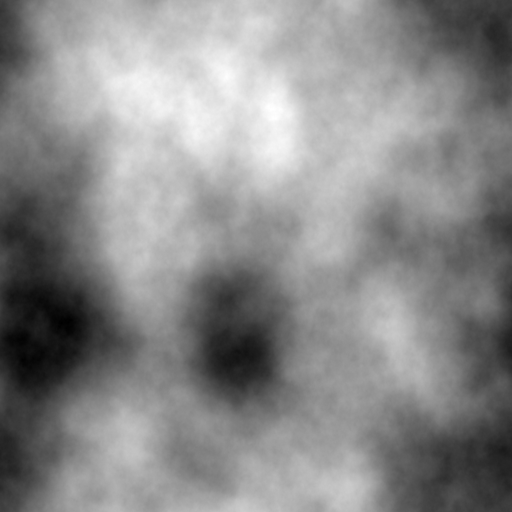
\includegraphics[width=0.3\columnwidth]{figures/u_30_500km_heights.png}
					 }
					 \hfill
					 \subfloat[Displacement $X$]
					 {
					 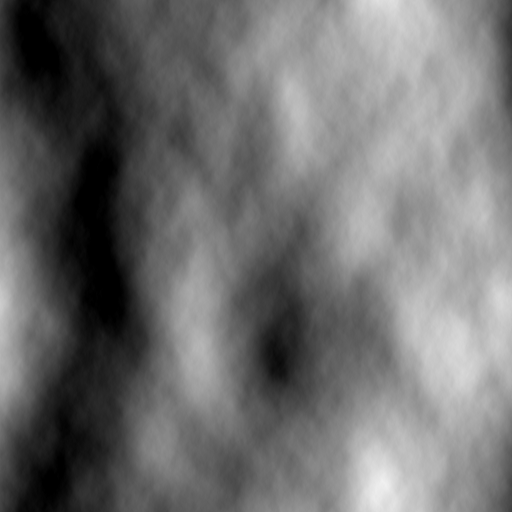
\includegraphics[width=0.3\columnwidth]{figures/u_30_500km_displacement_x.png}
					 }
					 \hfill
					 \subfloat[Displacement $Z$]
					 {
					 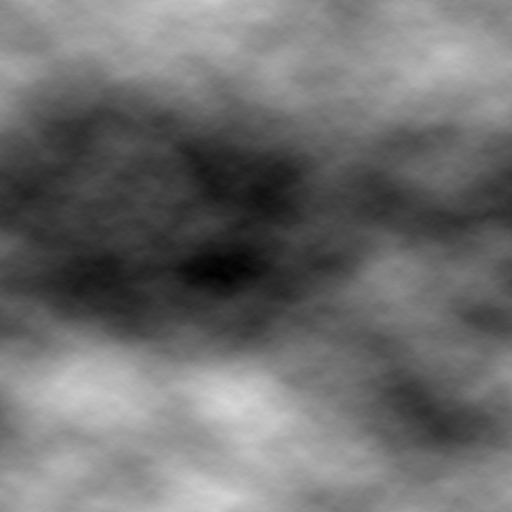
\includegraphics[width=0.3\columnwidth]{figures/u_30_500km_displacement_z.png}
					 }
					\end{figure}
				\end{column}	  
			\end{columns}
		\end{block}
	\end{minipage}
	\begin{minipage}{0.99\textwidth}
		\begin{block}{Ocean Surface Rendering}
			\begin{columns}[t]
				\begin{column}{0.95\linewidth}
					\begin{figure}
					\centering
%					\noindent
					\subfloat[Triangle mesh\label{fig:a}]{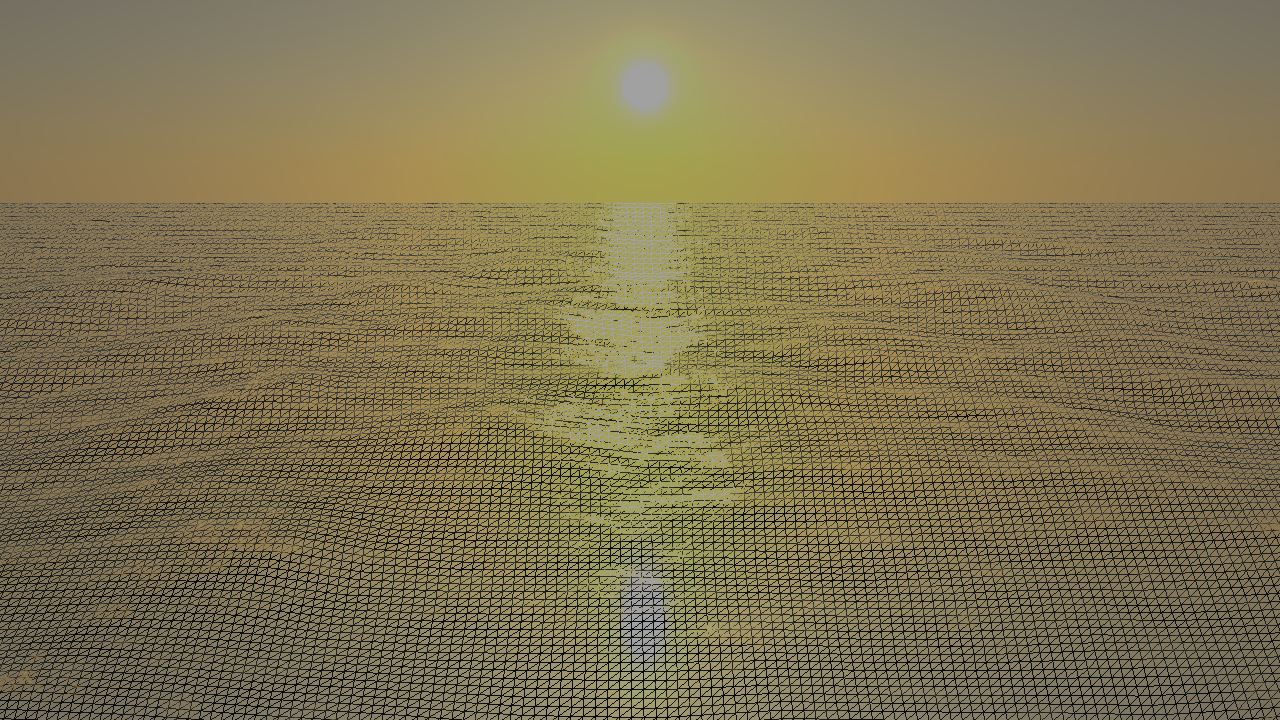
\includegraphics[width=0.165\columnwidth]{figures/28-05-2018_10-56-10_grid}}
					\subfloat[Reflected sun light\label{fig:b}]{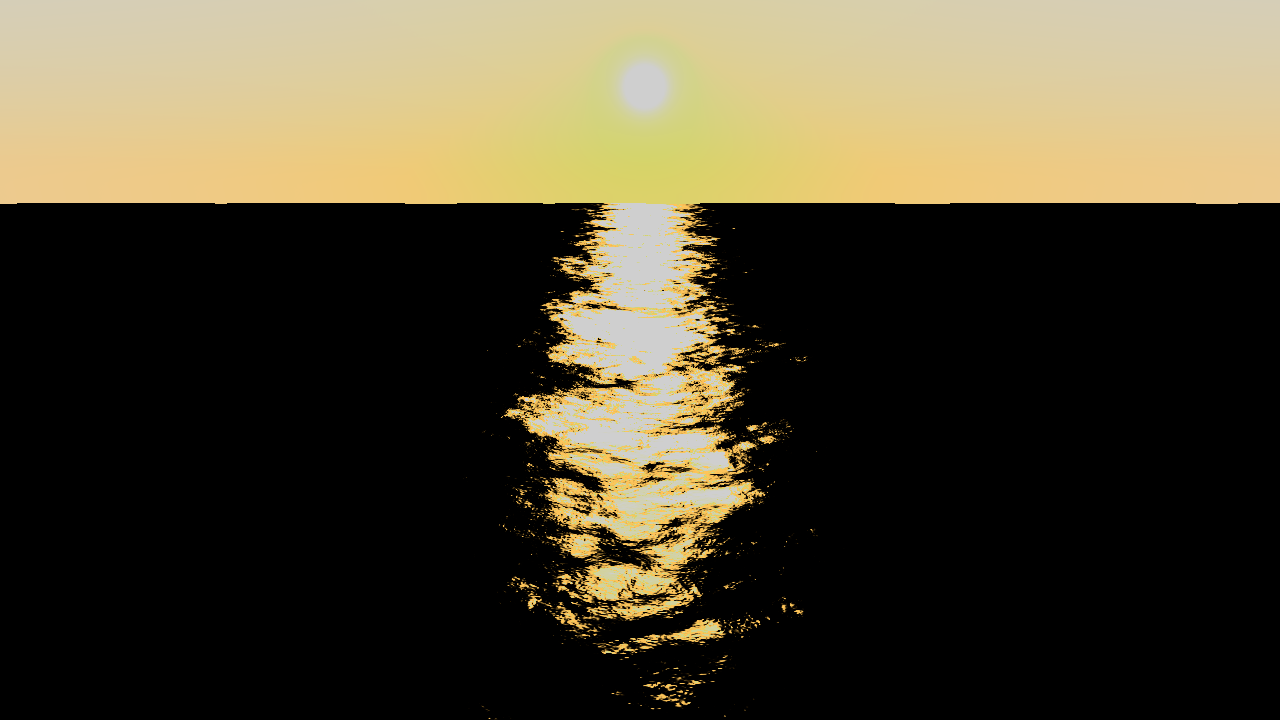
\includegraphics[width=0.165\columnwidth]{figures/28-05-2018_10-56-10_ross}}
					\subfloat[Reflected sky light\label{fig:c}]{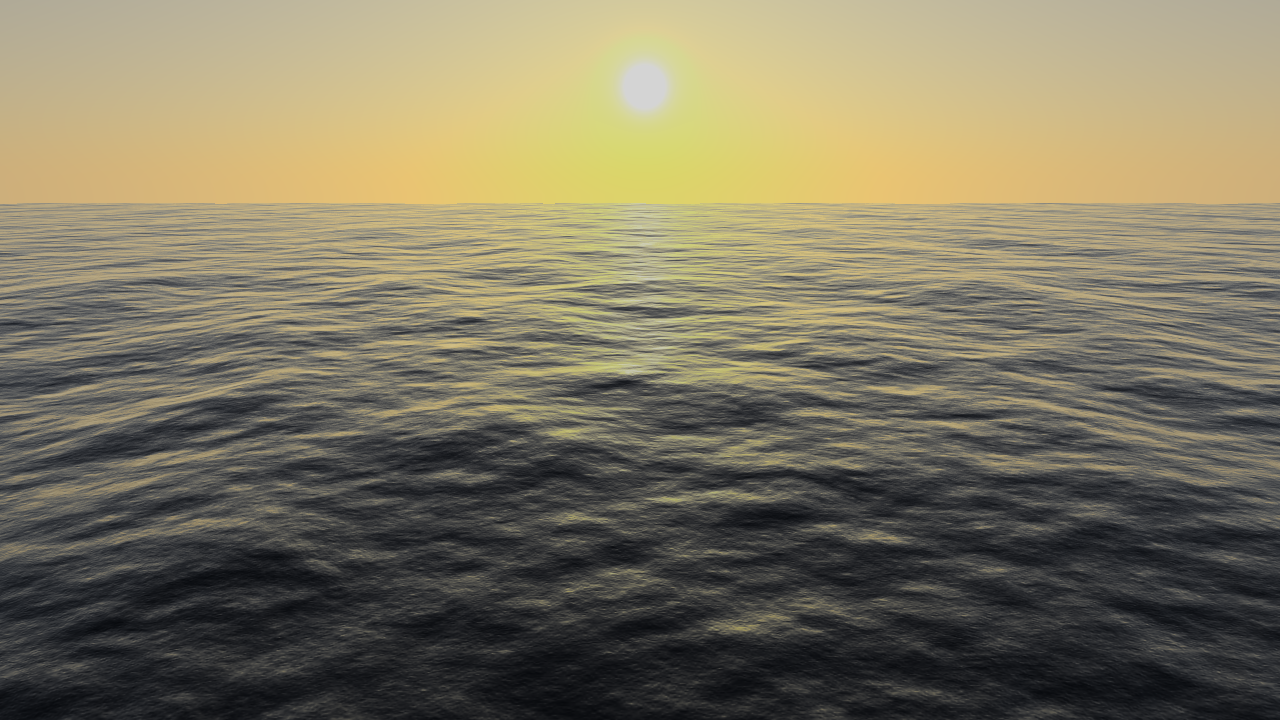
\includegraphics[width=0.165\columnwidth]{figures/28-05-2018_10-56-10_sky}}
					\subfloat[Refracted light \label{fig:d}]{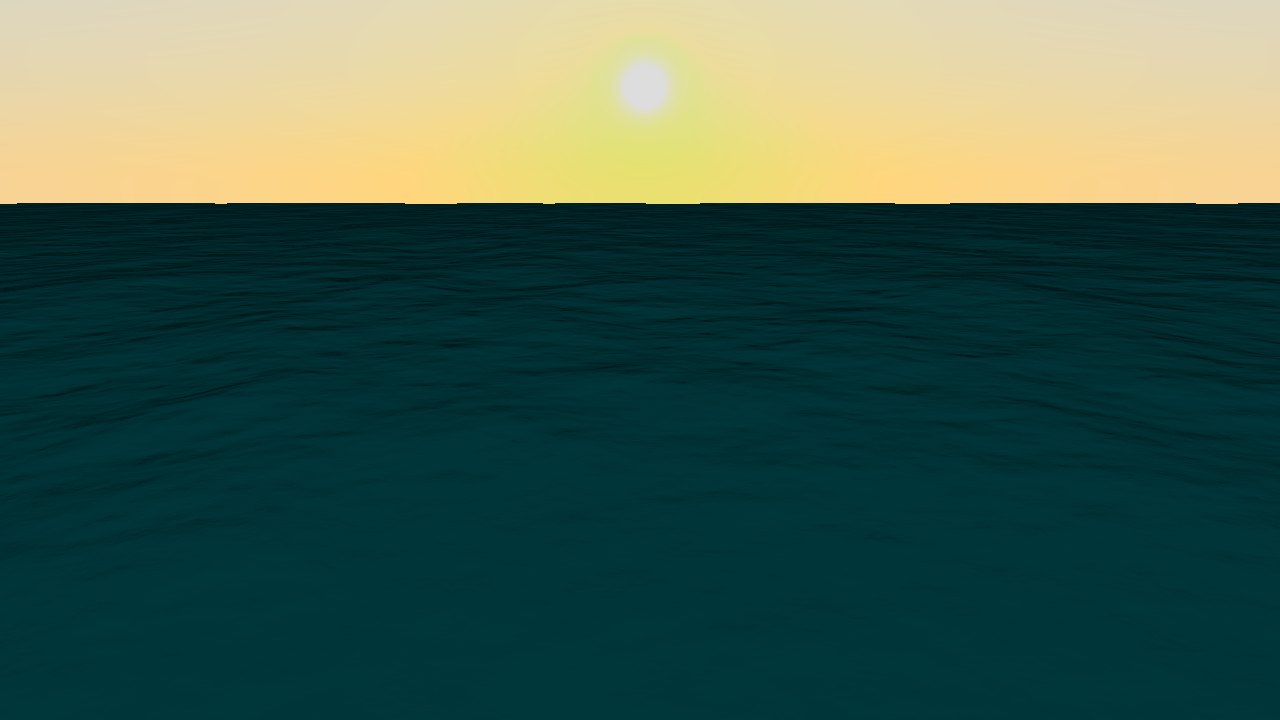
\includegraphics[width=0.165\columnwidth]{figures/28-05-2018_10-56-10_sea}}
					\subfloat[Whitecap foam\label{fig:e}]{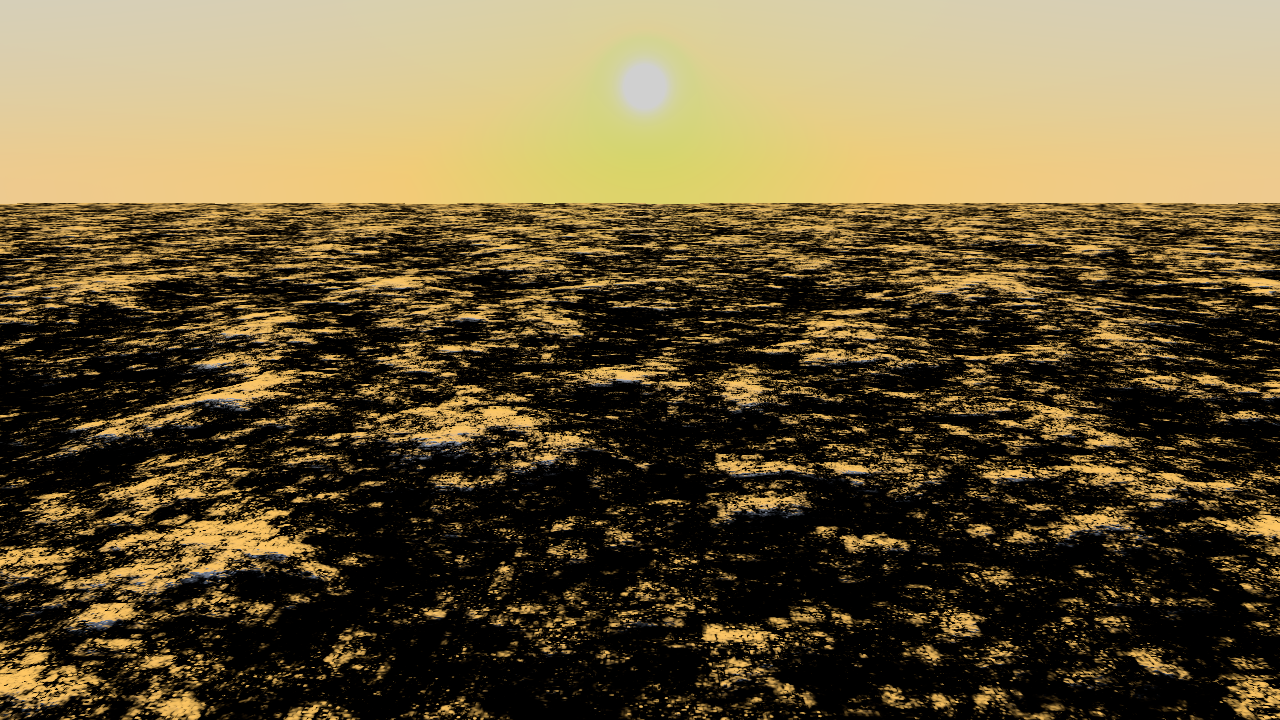
\includegraphics[width=0.165\columnwidth]{figures/28-05-2018_10-56-10_whitecaps}}
					\subfloat[Final result\label{fig:f}]{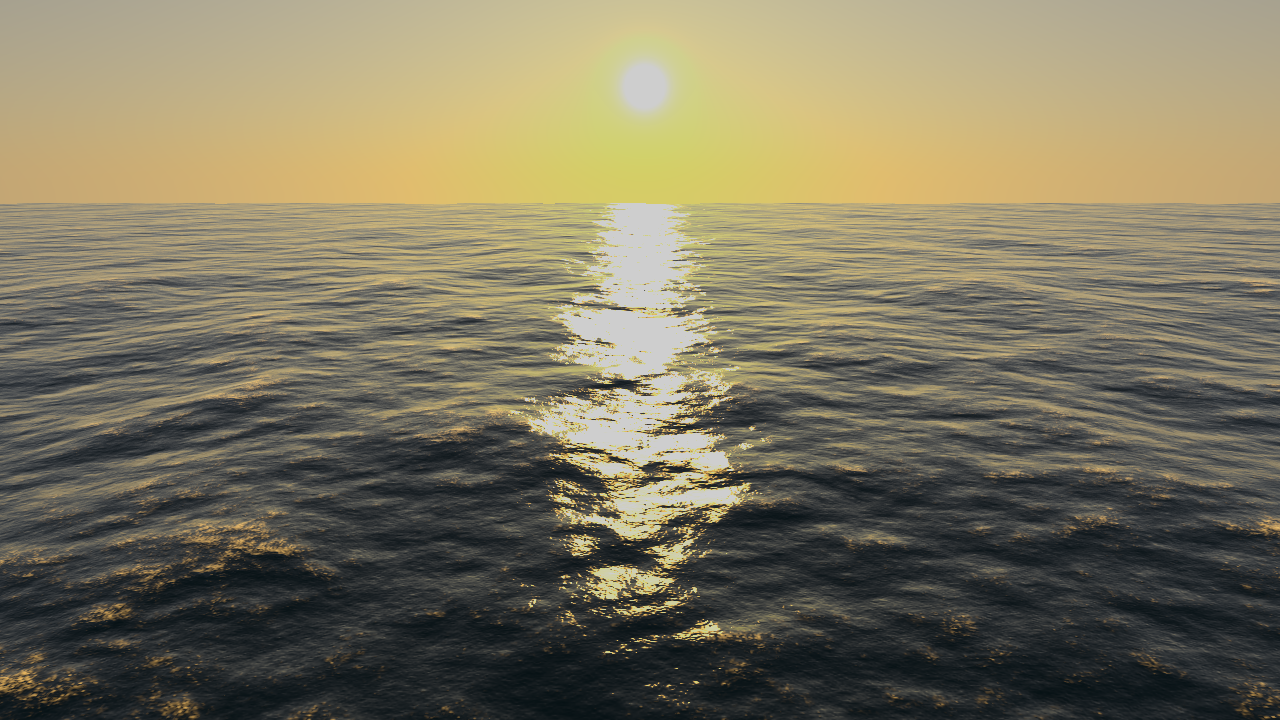
\includegraphics[width=0.165\columnwidth]{figures/28-05-2018_10-56-10_complete}}
					\end{figure}
%					\vspace{0.5cm}
%					\begin{center}
%					From left to right: \subref{fig:a}
%					\end{center}
				\end{column}
%				\begin{column}{0.35\linewidth}
%					\subref{fig:a} The adaptive, constant-overhead mesh
%					
%					\subref{fig:b} Sun light reflected by the water surface
%					
%					\subref{fig:c} Sky light reflected by the water surface
%					
%					\subref{fig:d} Light refracted from the water body				
%					
%					\subref{fig:e} Whitecap foam
%					
%					\subref{fig:f} The final result
%				\end{column}				
			\end{columns}
		\end{block}
	\end{minipage}
	\begin{minipage}{0.99\textwidth}
		\begin{block}{Results}
			\begin{columns}[t]
				\begin{column}{0.4\linewidth}
				\begin{itemize}
				\item Generate and render the animated ocean surface in real time
				\item Seamless transition between close-ups and panoramas
				\item Supports a large variety of seas
				\item User controlled balance between model detail and performance
				\end{itemize}
				\end{column}
				\begin{column}{0.5\linewidth}
				\begin{figure}
				\centering
				\subfloat{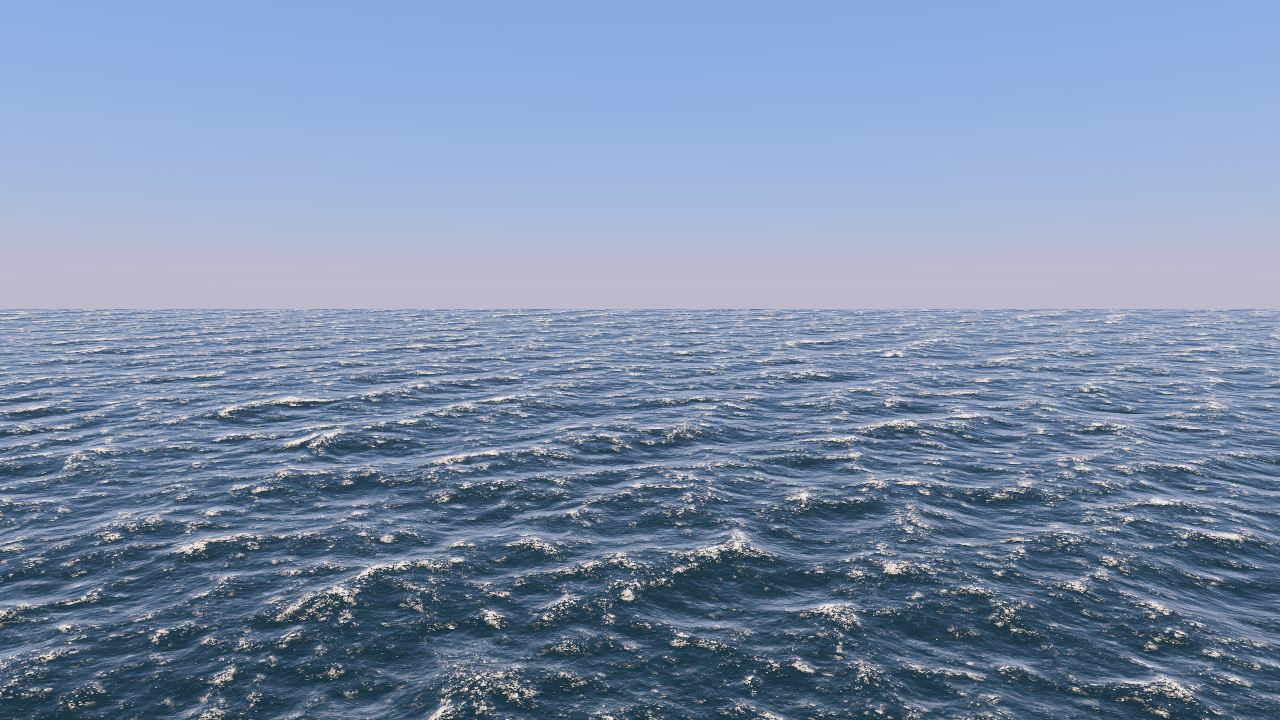
\includegraphics[width=0.32\columnwidth]{figures/21-06-2018_10-44-51_complete}}
				\hfill
				\subfloat{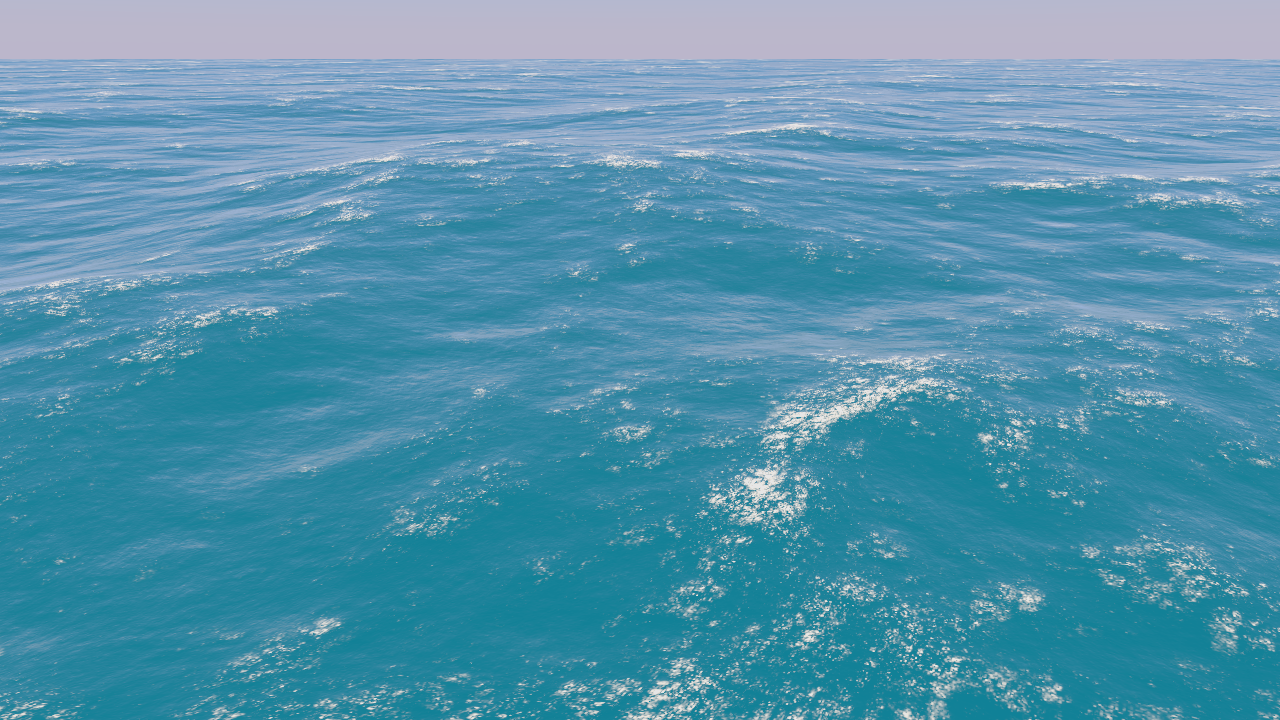
\includegraphics[width=0.32\columnwidth]{figures/21-06-2018_13-45-06_complete}}
				\hfill
				\subfloat{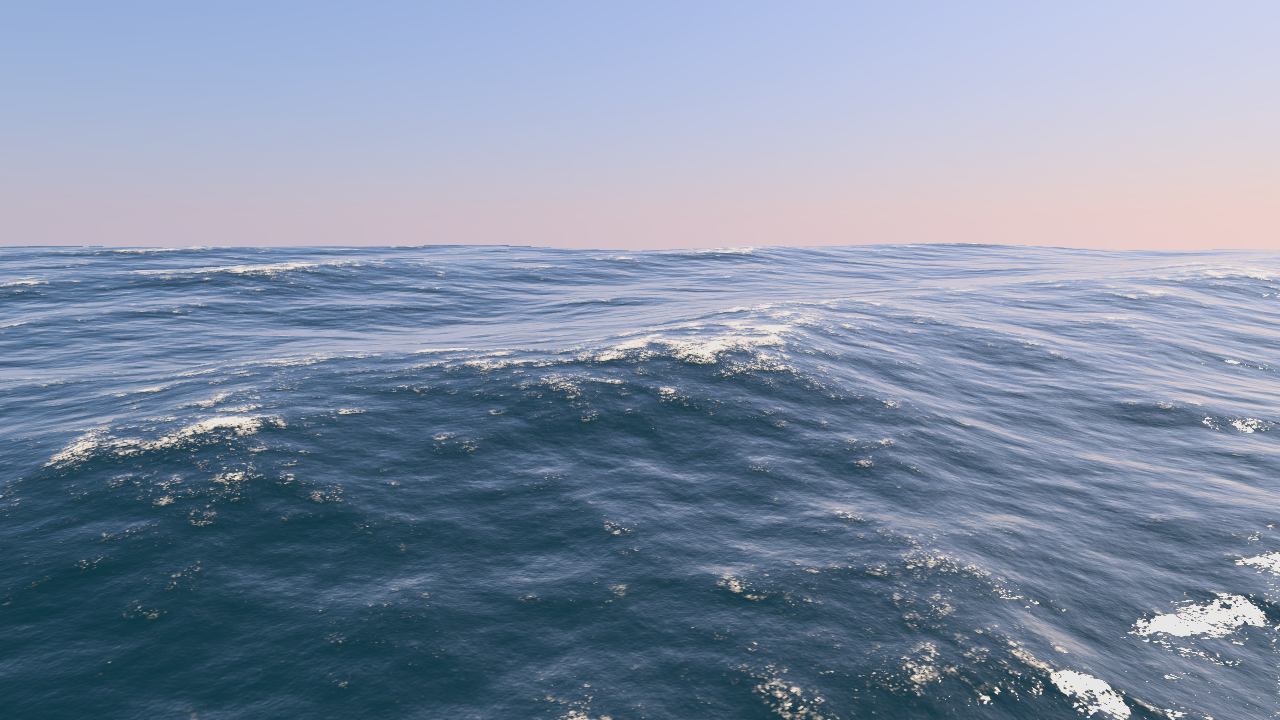
\includegraphics[width=0.32\columnwidth]{figures/21-06-2018_12-48-51_complete}}
				\end{figure}
%				\begin{center}
%				\noindent
%				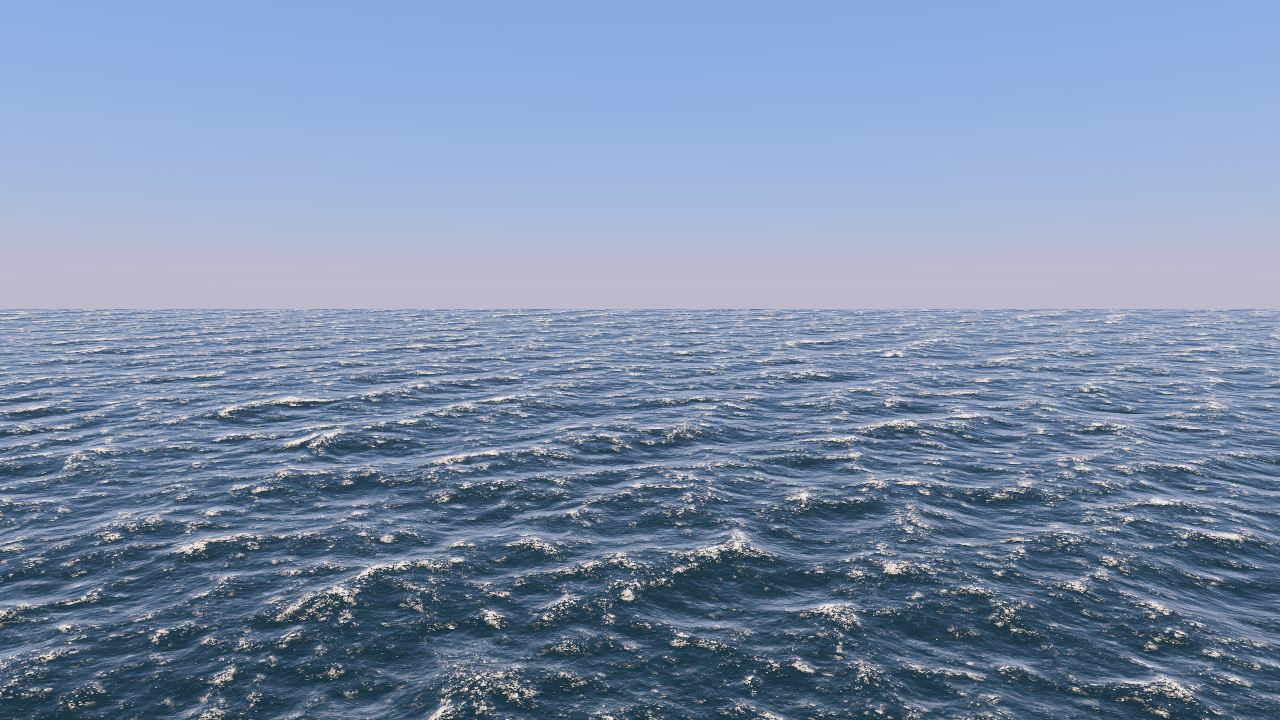
\includegraphics[width=0.32\columnwidth]{figures/21-06-2018_10-44-51_complete}
%				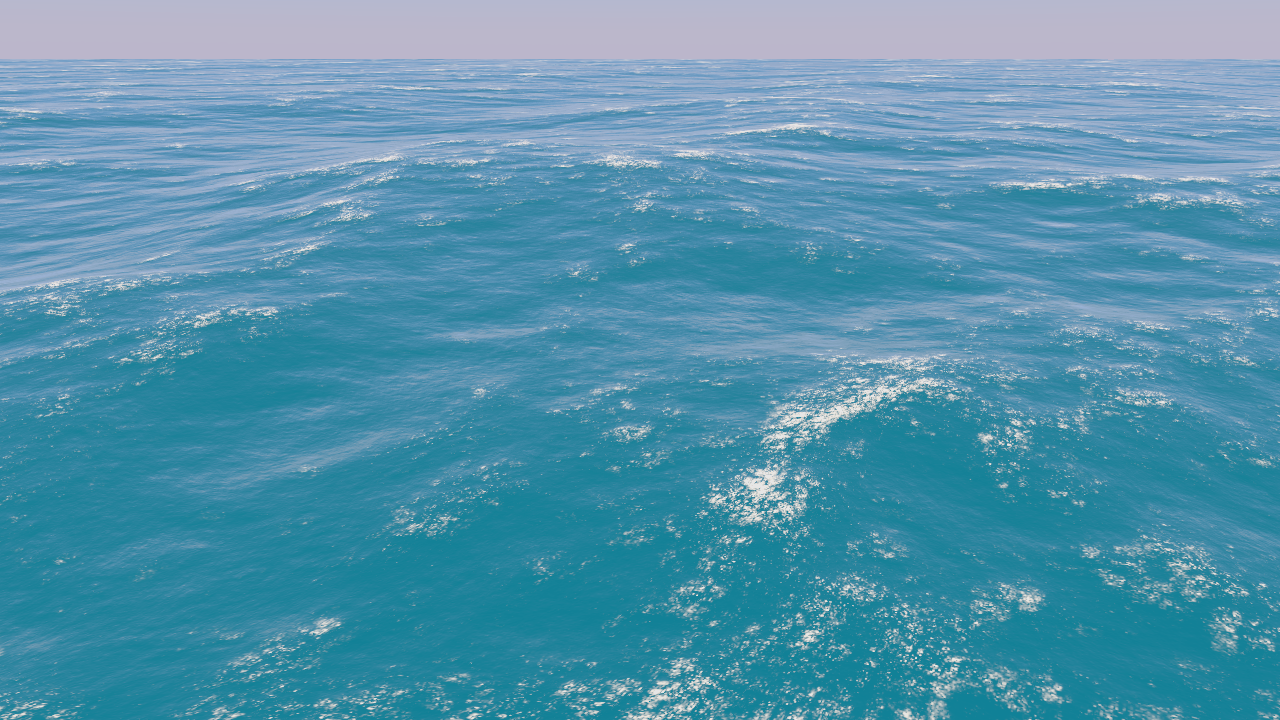
\includegraphics[width=0.32\columnwidth]{figures/21-06-2018_13-45-06_complete}
%				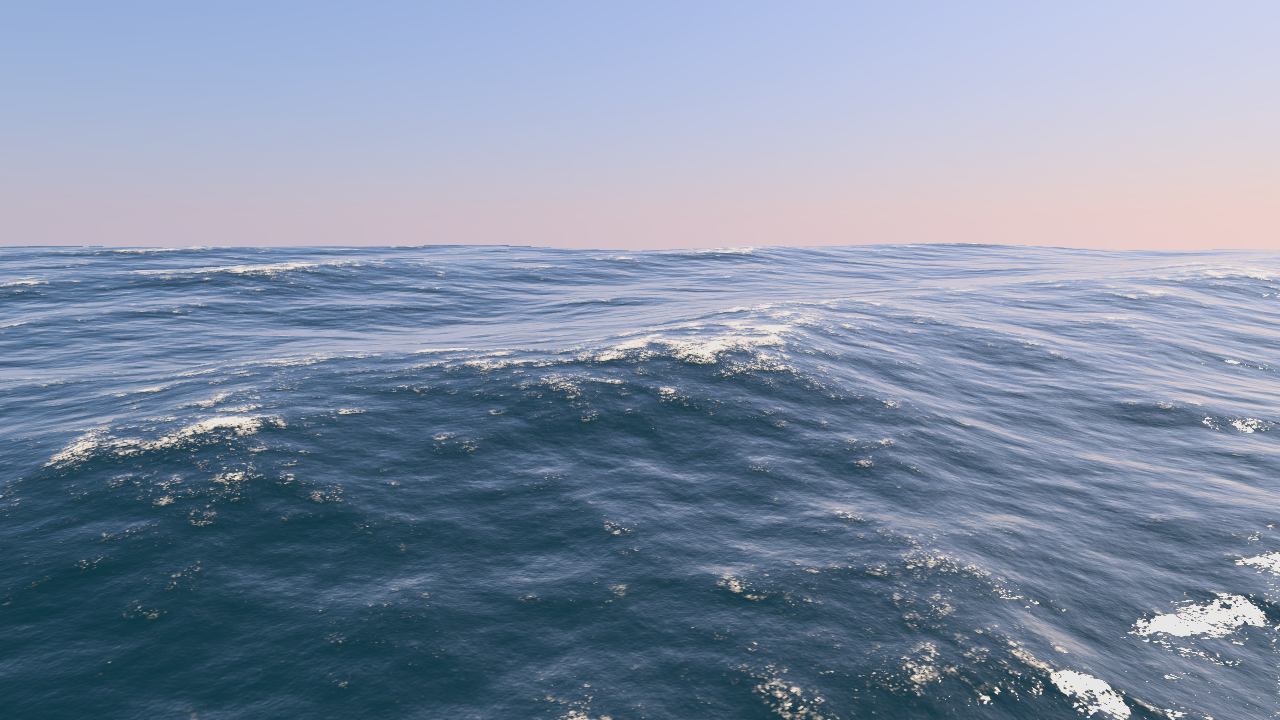
\includegraphics[width=0.32\columnwidth]{figures/21-06-2018_12-48-51_complete}
%				\end{center}
				\end{column}
			\end{columns}
		\end{block}
	\end{minipage}
	\begin{minipage}{0.99\textwidth}
		\begin{block}{References}
%			{\small
%			\setbeamertemplate{bibliography item}[text]
%			\bibliographystyle{plain}
%       		\bibliography{references}
%			}
%			\begin{center}
			\small
			\setbeamertemplate{bibliography item}[text]
%			\setlength{\columnsep}{0.1\linewidth}
			\begin{multicols}{2}
			\centering
			\bibliographystyle{plain}
			\bibliography{references}
			\end{multicols}
%			\end{center}
		\end{block}
	\end{minipage}
	\end{center}
%    \begin{varblock}[0.975\textwidth]{Introduction}
%    \end{varblock}
%    \begin{varblock}[0.975\textwidth]{Ocean Surface Generation}
%    Brak
%    \end{varblock}
%    \begin{varblock}[0.975\textwidth]{Ocean Surface Rendering}
%    Brak
%    \end{varblock}
%    \begin{varblock}[0.975\textwidth]{Results}
%    Brak
%    \end{varblock}    
    
%  \begin{columns}[t]
%    % ---------------------------------------------------------%
%    % Set up a column
%    \begin{column}{.45\textwidth}
%      
%    \end{column}
%    % ---------------------------------------------------------%
%    % end the column
%
%    % ---------------------------------------------------------%
%    % Set up a column 
%    \begin{column}{.45\textwidth}
%      
%    \end{column}
%    % ---------------------------------------------------------%
%    % end the column
%  \end{columns}
%
%
%    \begin{thebibliography}{999}
%      
%    \bibitem[Foo~and~Fu, 2010]{ff2010}
%      Foo, B.; and Fu, B.
%      2010.
%      \newblock {On logical representations of hackerisms}.
%      {\em J.~Log.~Hack.} 1:1--2.
%      
%    \bibitem[Crock~et~al., 2010]{ck2010}
%      Crock, A; Cruft, B.; and Kludge, C.
%      2010.
%      \newblock {Decomposing junk code}.
%      Manuscript.
%      
%    \end{thebibliography}

\end{frame}

\end{document}

%%% Local Variables:
%%% TeX-PDF-mode: t
%%% TeX-debug-bad-boxes: t
%%% TeX-master: t
%%% TeX-parse-self: t
%%% TeX-auto-save: t
%%% reftex-plug-into-AUCTeX: t
%%% End:
